%!TEX root = cahier_charges_afnor.tex
\section{Cadre de réponse}

%\subsection{Pour chaque fonction}

%\subsubsection{Solution proposée}
%%\subsubsection{Niveau atteint pour chaque critère d’appréciation de cette fonction et modalités de contrôle}
%%\subsubsection{Part du prix attribué à chaque fonction}


%\subsection{Pour l’ensemble du produit}

%%\subsubsection{Prix de la réalisation de la version de base}
%\subsubsection{Options et variantes proposées non retenues au cahier des charges}
%
%\subsubsection{Mesures prises pour respecter les contraintes}
% et leurs conséquences économiques}
% Hibernate ? sql? 

Un prototype de l'interface permettant d'en percevoir la conception générale est proposé figure~\ref{fig:archi}.

\subsubsection{Outils d’installation, de maintenance}

\begin{figure}[htbp]
	\centering
		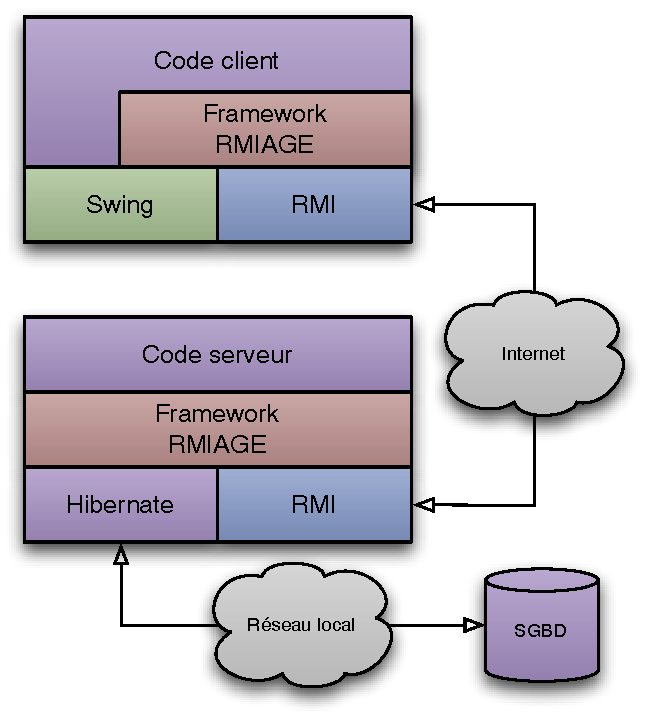
\includegraphics[scale=1]{../diagrammes/architecture.pdf}
	\caption{Architecture}
	\label{fig:archi}
\end{figure}

Le produit sera livré sous forme d'archives JAR contenant la librairie et les programmes témoins.

Les instructions concernant la configuration d'Hibernate seront également fournies.

%\subsubsection{Décomposition en modules, sous-ensembles}
%\subsubsection{Prévisions de fiabilité}
%\subsubsection{Perspectives d’évolution technologique}

